\documentclass[addpoints,12pt]{exam}
\usepackage{multicol}
\usepackage{arev}
\usepackage{graphicx,multicol}
\usepackage[euler-digits]{eulervm}
\usepackage{charter,amsmath,amssymb}
\usepackage[letterpaper,margin=1in]{geometry}
\pagestyle{headandfoot}
\runningheadrule
\firstpageheader{\bf Math 104}{\bf Exam 2, Red Form}{\bf 8 October 2014}
\runningheader{\bf Math 104}
{\bf Exam Two, Page \thepage\ of \numpages}
{\bf 8 October 2014}
\firstpagefooter{}{}{}
\runningfooter{}{}{}
\begin{document}

\begin{center}
\fbox{\fbox{\parbox{5.5in}{
This section has \numquestions~questions.
It has been printed on \numpages~pages and is worth \numpoints~points.
Answer all the questions below in the spaces provided.
In order to receive maximum credit, you must
clearly indicate how you arrived at your answers.
By signing below, you pledge that you
\begin{enumerate}
\item will not communicate to any person in any conceivable way anything
about the contents of this exam
until all students have taken the exam, and
\item in taking this exam now,
you have not been the recipient of such communication from anyone else.
\end{enumerate}}}}
\end{center}
\vspace{.2in}
\makebox[\textwidth]{Your signature:\enspace\hrulefill}\\
\vspace{.2in}\\
\makebox[\textwidth]{Your name:\enspace\hrulefill}\\
\vspace{.2in}\\
\makebox[\textwidth]{Your student ID number:\enspace\hrulefill}\\

\begin{questions}

\question[10] Two dice are rolled and the
numbers on the top faces of the two dice are observed.
Determine the odds against each of the following events.
\begin{parts}
\part Both numbers are the same.
\vspace{.25in}
\part The sum of the two numbers is $5$.
\vspace{.25in}
\part The sum of the two numbers is even.
\vspace{.25in}
\end{parts}

\question[10]
\begin{multicols}{2}
When dropping a thumbtack, it either lands point down
or point up, as shown in the image at the right.
Alex drops all the thumbtacks in a box on the floor.
$106$~tacks land point down, while $35$ land point up.
Based on these results, if he drops two thumbtacks, what
is the probability that both tacks will land point up?
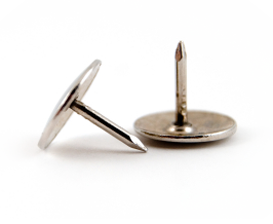
\includegraphics[scale=.5]{Thumbtacks}
\end{multicols}

\question[10] Expectation of new game

\question[10] Suppose $E$ and $F$ are events
and $P\left(E\right)=.75$ and $P\left(F\right)=.25$.
\begin{parts}
\part Calculate $P\left(\text{$E$ or $F$}\right)$
assuming that $E$ and $F$ are mutually exclusive.
\part Calculate $P\left(\text{$E$ and $F$}\right)$
assuming $E$ and $F$ are independent.
\part Calculate $P\left(\text{$E$ or $F$}\right)$
assuming $E$ and $F$ are independent.
\end{parts}

\question Ames High School has
$156$ students in band and $34$
students in both band and chorus.
If $1089$ of the $1422$ students at Ames High
are in neither band nor chorus, how many students
are in chorus?

\question[10] Alex, Brooke, Colby, and Denise comprise
the student council. They want to select a president,
a vice president, and a treasurer from among themselves.
However, Alex and Denise cannot serve together in any two
of these roles because they dislike each other.
\begin{parts}
\part How many possible choices of president, vice president,
and treasurer are there?
\part In how many choices does Alex appear in some role?
\part What is the probability that Brooke will be chosen
for president, vice president, or treasurer?
\end{parts}

\question[10] If two cards are randomly selected from a deck
of playing cards, what is the probability that both cards
will be picture cards?
A {\em picture card} is either a Jack, Queen, or King.

\question[10] To raise money the volleyball team sells 500~raffle tickets
for $\$3$ each. They will randomly select a ticket holder to receive
a prize. If the fair ticket price is $0.30$, how much is the prize?

\end{questions}

\vfill
\begin{center}\gradetable[h][questions]\end{center}

\end{document}
